\documentclass{standalone}
\usepackage{tikz}
\usetikzlibrary{arrows.meta, positioning, shapes}

\begin{document}

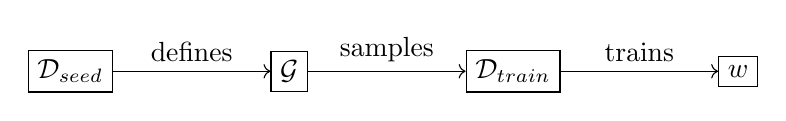
\begin{tikzpicture}[node distance=2cm, auto]
    \node [rectangle, draw] (data) {$\mathcal{D}_{\text{seed}}$};
    \node [rectangle, draw, right=of data] (g) {$\mathcal{G}$};
    \node [rectangle, draw, right=of g] (dt) {$\mathcal{D}_{\text{train}}$};
    \node [rectangle, draw, right=of dt] (w) {$w$};

    \draw[->] (data) -- node [above] {defines} (g);
    \draw[->] (g) -- node [above] {samples} (dt);
    \draw[->] (dt) -- node [above] {trains} (w);
\end{tikzpicture}

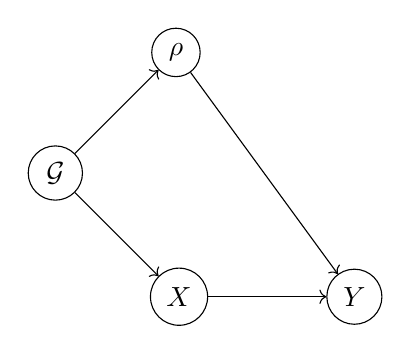
\begin{tikzpicture}[node distance=1.5cm, auto]
    \node [circle, draw] (g) {$\mathcal{G}$};
    \node [circle, draw, above right=of g] (rho) {$\rho$};
    \node [circle, draw, below right=of g] (x) {$X$};
    \node [circle, draw, right=of x] (y) {$Y$};

    \draw[->] (g) -- (rho);
    \draw[->] (g) -- (x);
    \draw[->] (rho) -- (y);
    \draw[->] (x) -- (y);
\end{tikzpicture}

Left: Data generation pipeline. Right: The fine-tuned network \( q_\theta \) learns to do inference in a graphical model where the prior over programs, \( \mathcal{G} \), is defined by prompting an LLM with example code in \( \mathcal{D}_{\text{seed}} \), while the likelihood \( p(Y | \rho, X) \) is defined by program execution.

\end{document}